\documentclass{article}

\setlength{\topmargin}{0pt}
\setlength{\oddsidemargin}{0pt}
\setlength{\evensidemargin}{0pt}
\setlength{\textwidth}{6in}
\setlength{\voffset}{0pt}
\setlength{\headheight}{0pt}
\setlength{\headsep}{0pt}
\setlength{\textheight}{9in}

\usepackage{amsmath}
\usepackage{latexsym}
\usepackage{amssymb}
\usepackage{graphicx}



\newcommand{\vect}{\vec}
\newcommand{\lp}{\left(}
\newcommand{\rp}{\right)}
\newcommand{\lb}{\left[}
\newcommand{\rb}{\right]}
\newcommand{\lc}{\left\{}
\newcommand{\rc}{\right\}}t
\newcommand{\lab}{\left|}
\newcommand{\rab}{\right|}
\newcommand{\la}{\left\langle}
\newcommand{\ra}{\right\rangle}
\DeclareMathOperator{\curl}{curl}
\DeclareMathOperator{\diver}{div}
\newcommand{\bR}{\mathbb{R}}
\newcommand{\Nat}{\mathbb{N}}
\newcommand{\sB}{\mathcal{B}}
\newcommand{\sC}{\mathcal{C}}
\newcommand{\sF}{\mathcal{F}}
\renewcommand{\phi}{\varphi}
\DeclareMathOperator{\Real}{Re}
\DeclareMathOperator{\Imag}{Im}
\newcommand{\Rq}{\Rightarrow\quad}

\newcommand{\ihat}{\vect{\imath}}
\newcommand{\jhat}{\vect{\jmath}}
\newcommand{\khat}{\vect{k}}


\DeclareMathOperator{\KE}{KE}
\DeclareMathOperator{\PE}{PE}
\DeclareMathOperator{\TE}{TE}



\begin{document}

\begin{center}
\LARGE
Homework \#1
\normalsize

\bigskip
Math 263, Spring 2022

{\bf Due Thursday, February 3.}

\bigskip
\end{center}


\normalsize

\begin{enumerate}

\item
\begin{enumerate}
\item How many different anagrams of the word ZOOKEEPER are possible?
\item How many different anagrams of the word ZOOKEEPER are possible if the first and last letters in the anagram must be the same?
\end{enumerate}


\bigskip

\item A club has 9 members, 3 of whom are sisters. The club members need to line up in a row for the club photograph. How many ways can they line up (that is, in how many different orders can they stand, say, from left to right) if the 3 sisters want to stand together?


\bigskip


\item A group of 6 women and 5 men must form a 5-person committee, consisting of a chair, a vice-chair, and 3 at-large members. 
\begin{enumerate} 
\item How many different ways are there to form this committee, if the chair and vice-chair must be of different genders? 
\item How many different ways are there to form this committee, if the chair and vice-chair must be of the same gender? (This is a strange policy, but that doesn't mean we can't compute the answer.)
\end{enumerate}
\bigskip


\item Suppose a club has 8 members, 2 of whom are brothers. The club needs to form a 4-person committee. How many ways can this committee be formed, if there is a rule that no one on the committee can be related to anyone else on the committee?

\bigskip

\item Consider the grid below. A step consists of walking from one lattice point to an adjacent lattice point (along the line joining them). A shortest path (one consisting of the minimum possible number of steps) from point $A$ (the lower-left corner) to point $B$ (the upper-right corner) consists of 6 steps, but such a path is not unique. (A standard way to think of such a grid is as streets in a city, where of course you can only drive from one intersection to another by following the streets.)
\bigskip
\bigskip
\begin{center}
 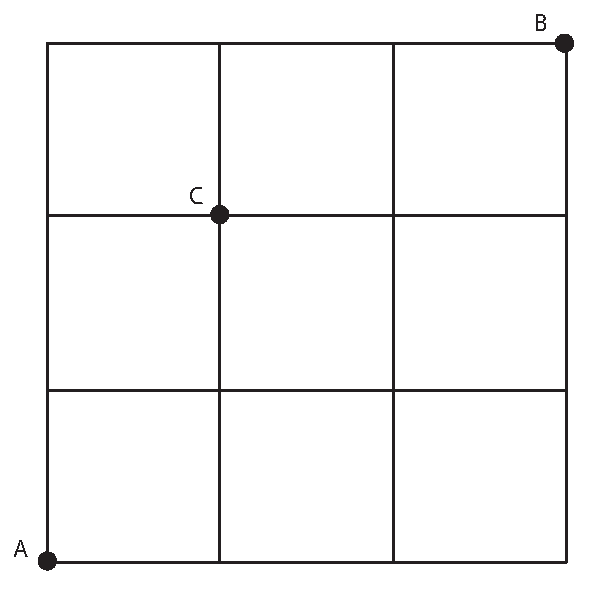
\includegraphics[width=4in]{Drawing1.pdf}
\end{center}

\begin{enumerate}
\item How many shortest paths from $A$ to $B$ are there?
\item Suppose that a path is not allowed to pass through point $C$. (Thinking about driving through a city, this would correspond to the intersection being closed, say, for road work.) Now how many shortest paths from $A$ to $B$ are there?
\item For any positive integer $n$, give a combinatorial proof of the identity
\[
\binom{2n}{n} = \sum_{i=0}^n \binom{n}{i}\binom{n}{n-i}
\]
\emph{Hint:} Think about an $n\times n$ grid, and where you might be halfway on your path from the lower-left corner to the upper-right corner.
\end{enumerate}



\end{enumerate}

\end{document}